%-------------------------------------------------------------------------------------------------%
% A related work section in which the relevant literature is presented and 
% linked to the project. 
% It should show that you clearly know the problem you plan to solve, 
% and that you master the related work. 

% The environment proposed by this thesis builds from Ravi Peter's work. GeoFront can be seen as GeoFlow, but in a web browser. However, the introduction of this web component significantly changes the purpose and use-case of GeoFront compared to GeoFlow. 

% GeoFlow's mission: Create a geoprocessing pipeline in a visual environment, in order to speed up and improve the quality of the development process of this pipeline "FOR YOURSELF", compared to text-based methods. This speed and quality comes from the fact that the visual environment makes rapid experimentation and evaluation possible. This is especially helpful for non-determinant processes, or processes containing 'magic' number parameters. Examples of these are RANSAC algorithms. 

% GeoFront's mission: Use the vpl to make rapid experimentation and evaluation of your geoprocessing functions possible FOR OTHERS. This enables others to rapidly utilize your geoprocessing method. The primary use case of this is collaboration: Rapidly publish ones results, demonstrate reproducibility, retrieve feedback, etc.   

\chapter{Related work}
\label{chap:related}

This chapter offers an overview of the theoretical background that this study builds upon, alongside a review of related studies. 
The study takes place at the intersection of the two fields of Visual programming and web GIS applications. 
This is why this chapter is divided into three sections. \refsec{sec:vp} and \refsec{sec:webgis} each cover one of these fields individually, and \refsec{sec:both} covers comparable studies at this intersection.

Every section is structured in the same manner. Each starts out with a general background on the field in question, after which an overview of comparable studies is given. It ends with a review, which compares these studies with the main research question. This is done to specify exactly how these prior studies relate to the research question, vital in explaining the decisions of sub-questions and the methodology.

%%%%%%%%%%%%%%%%%%%%%%%%%%%%%%%%%%%%%%%%%%%%%%%%%%%%%%%%%%%%%%%%%%%%%%%%%%%%%%%
%%%%%%%%%%%%%%%%%%%%%%%%%%%%%%%%%%%%%%%%%%%%%%%%%%%%%%%%%%%%%%%%%%%%%%%%%%%%%%%
%%%%%%%%%%%%%%%%%%%%%%%%%%%%%%%%%%%%%%%%%%%%%%%%%%%%%%%%%%%%%%%%%%%%%%%%%%%%%%%
\section{Visual Programming}
\label{sec:vp}

\subsection*{BACKGROUND}

offers a rich background of prior research, and as such this literature review cannot be exhaustive. We instead focus on works which are particularly relevant to this studies' problem statement.


\begin{lstlisting} 
write something about : 
- cognitive_1996 
- advances_2004
- characterizing_2021

An increasing number of software applications are being written by end users 
without formal software development training. 
This inspired large technology companies such as Microsoft [91] and Amazon [90] 
to invest in low-code development environments empowering end users to 
create web and mobile applications. 
According to the 2019 Q1 Forrester report, the low-code market will witness an 
annual growth rate of 40\%, 
with spending forecast to reach \$21.2 billion by 2022 [102]. 
End-User Development (EUD) has emerged as a field that is concerned with 
tools and activities allowing end users 
who are not professional software developers to write software applications [11]. 
This is promising as end users know their own domain and needs more than anyone else, 
and are often aware of specificities in their respective contexts. 
Further, as end users outnumber developers with professional software development 
training by a factor of 30-to-1, 
EUD enables a much larger pool of people to participate in software development [12]. 
A visual programming language (VPL), among other EUD techniques, 
allows end users to create a program by piecing together graphical elements
 rather than textually specifying them [9]. 
Traditionally, visual programming has been successfully used to help novices
 learn basics of programming by visualizing elements of a program. 
However, visual programming is increasingly being used by end 
users in various domains to create and tailor applications that are useful 
beyond the realm of education. 
For instance, VPLs are now being used in fields such as 
the Internet of Things (IoT) [3], [10], mobile 
application development [51], robotics [8], and Virtual/Augmented Reality [4].
}

From characterizing_2021

other major use cases: 
- PLC: Ladder

\end{lstlisting}

%%%%%%%%%%%%%%%%%%%%%%%%%%%%%%%%%%%%%%%%%%%%%%%%%%%%%%%%%%%%%%%%%%%%%%%%%%%%%%%
\subsection*{Dataflow modelling}

\begin{lstlisting}
- Dataflow modelling is a field closely related to visual programming.
- However, where visual programming is concerned with many aspects, 
interface and usability being one of them, dataflow modelling is 
primairly concerned with the correct representation of data transformation.   
- within the field of dataflow modelling, it turned out that certain 
visual programming paradigms are advantageous, since they make parallel 
programming explicit. Thus, these fields are often named in conjunction. 
- The important take-away is that visual programming is not 
just a matter of UI or a stylistic choice.

- By more correctly representing dataflow and communicating 
opportunities for parallel computation, it can lead to faster applications.
\end{lstlisting}


%%%%%%%%%%%%%%%%%%%%%%%%%%%%%%%%%%%%%%%%%%%%%%%%%%%%%%%%%%%%%%%%%%%%%%%%%%%%%%%
\subsection*{ In Geometry Computation \& Visualization }
\begin{lstlisting} 
   - Besides the use cases already mentioned, a significant number of 
   visual programming applications are emerging in fields concerned 
   with 2D and 3D geometry creation \& visualization. 

  PROCEDURAL GEOMETRY 
    - Rhino: Grasshopper
    - Revit: Dynamo  
    - Blender: Geometry Nodes
    - Houdini: Procedural Modelling
  
  TEXTURES AND SHADERS
    - Blender: Shader Nodes
    - Adobe: Substance Designer
    - Unreal Engine: Material Nodes
    - Unity: Shader Graph
    - Houdini: FX

  These are all popular applications, many users, multiple courses and tutorials, 

  The persistence of visual programming within the field of shaders and
  geometry, suggests that visual programming languages are advantageous in
  situations where a 'visual' product requires debugging during development. 
\end{lstlisting}



%%%%%%%%%%%%%%%%%%%%%%%%%%%%%%%%%%%%%%%%%%%%%%%%%%%%%%%%%%%%%%%%%%%%%%%%%%%%%%%
\subsection*{ In field of geo-informatics }

\begin{lstlisting}
  (explain the use-case of vpl's within the field of geo-informatics, 
  why they are significant to us) 
  within geomatics

  - data translation: FME 
  - cloud-native computation: modellab in rasterfoundry
    - link to dataflow modelling
  - debugging & experimentation: GeoFlow 
  
\end{lstlisting}

% Visual programming environment for geo-computation (geo-vpl) has been tried before, natively ( Grasshopper , FME , GeoNodes , Blender Geometry Nodes ). 


% The entire application runs client-side in a browser, and uses a visual programming language as its primary \ac{gui}.
% The main goal and feature of geofront is to take existing low level geo-computation libraries, and to make these interactively usable on the web. 
% These libraries include a limited set of CGAL operations, complied from C++, and various geo-computation algorithms such as Startin, written in Rust. 
% Being a visual programming language, GeoFront can be used to interactively alter the geodata pipeline. 
% In between products can quickly be inspected using a 3D viewer.

% We test how well contemporary web technologies support such an application, as well as judge aspects such as accessibility \& performance of said application. We also judge if this type of application is indeed beneficial and usable as a scripting / demo environment.  

% These features could all be implemented by normal means ( buttons, panels, sliders ) -->

% CHOICE: do something in-between python bindings, and a full fletched end-user application. 
% Ergo: Visual programming

% For input, the environment offers \ac{wms} and \ac{wfs} support, as well as ways for users to load locally stored geodata. Parameters can be specified using various ui components, such as sliders. 
% For output, the environment can be used to either save data to the user's local machine, or to visualize the results within the geofront application using a WebGL based viewport.

% Where ModelLab is build on top of recent improvements to the accessability of satellite imagery, GeoFront is build in anticipation to a similar development for point cloud datasets with the introduction of COPC.  The focus of Geofront is therefore on point cloud processing, and point-cloud based modelling, such as Digital Terrain Models (DTM). 

%%%%%%%%%%%%%%%%%%%%%%%%%%%%%%%%%%%%%%%%%%%%%%%%%%%%%%%%%%%%%%%%%%%%%%%%%%%%%%%
\newpage
\subsection*{REVIEW}
Challenges
\begin{lstlisting}
  - several challenges exist within the research field of visual programming. 
  - literature study (knowling what is and isnt being researched)
  - based upon : prior meta-analysis of 'characterizing_2021'
\end{lstlisting}

\subsubsection*{Difficulty in assessment of 'usability'}
\begin{lstlisting}
  - usability is a nebulous phenomenon, hard to measure empirically.
  - no consensus on evaluation frameworks among VPL researchers. 

  BUT (leave this part, mention it later)
  - we will make no such attempt. usability serves as background motivation. 
  - this study assumes vpl's are 'in general' more usable to end-users 
  than text-based alternatives, based on the positive results of most of the 
  studies analysed by communicating_2021.   
\end{lstlisting}


\subsubsection*{web based visual programming is underresearched}
\begin{lstlisting}
  
  large challenge
  - not many examples
    of these examples: 
    - no suitable starter projects
    - none are concerned with geometry

    - Visual programming environment for geo-computation 
    \emph{in a browser} has not been tried before. 


    "Finally, 53.3% (16) of the tools were available publicly with some documentation. 
    We strongly recommend that future tools are made available for end users as well as comprehensive documentation to ensure tool adoption and sustainability." communicating_2021 
   -> not fully related, but making this vpl web-based could seriously help this aspect of vpl assessment.   

\end{lstlisting}


\subsubsection*{VPL availabilty and life cycle}
\begin{lstlisting}
Finally, (communicating_2021) names the 'life cycle' of apps created 
with the VPL as one of the most overlooked aspects within VPL research. 
- extend 
- debug
- publish
- run
\end{lstlisting}



%%%%%%%%%%%%%%%%%%%%%%%%%%%%%%%%%%%%%%%%%%%%%%%%%%%%%%%%%%%%%%%%%%%%%%%%%%%%%%%
%%%%%%%%%%%%%%%%%%%%%%%%%%%%%%%%%%%%%%%%%%%%%%%%%%%%%%%%%%%%%%%%%%%%%%%%%%%%%%%
%%%%%%%%%%%%%%%%%%%%%%%%%%%%%%%%%%%%%%%%%%%%%%%%%%%%%%%%%%%%%%%%%%%%%%%%%%%%%%%
\section{Web GIS}
\label{sec:webgis}

\todo{This is dated. this section includes many old introductions, and requires refinement.}

\subsection{BACKGROUND}


%%%%%%%%%%%%%%%%%%%%%%%%%%%%%%%%%%%%%%%%%%%%%%%%%%%%%%%%%%%%%%%%%%%%%%%%%%%%%%%
\subsubsection*{The Geoweb}
\label{sec:geoweb}


The Geoweb, or Geospatial Web, covers a broad collection of topics located at intersection of the field of geo-information and the web. A noteworthy study on the Geoweb is Van den Brink's phd titled "Geospatial Data on the Web". \cite{brink_geospatial_2018}. She claims that even though geodata is vital to a diverse range of applications and people, the ability to properly retrieve geodata remains almost exclusive to experts in the field. This is to the determent of all these applications and people, jeopardizing value, opportunity, and decision making. She makes this argument by using the concept of FAIR geodata. Coined by \cite{mark_d_wilkinson_fair_2016}, The FAIR principles are a collection of four assessment criteria used to judge the usability of (scientific) data: Findable, Accessible, Interoperable, and Reusable. 

We argue that if these concerns count for geodata \textit{retrieval}, they should just as well count for geodata \textit{processing}. After all, if a user is unable to convert the retrieved geodata to their particular use case, then the information they seek remains inaccessible. Therefore, this study introduces the concept of \emph{FAIR geoprocessing}. 

Based on the arguments presented by \cite{brink_geospatial_2018}, we can also extrapolate that a \ac{gis} environment shouldn't exclusively be used by only experts. Van den Brink mentions a group called 'data users', presented as "web developers, data journalists etc. who use different kinds of data, including geospatial data, directly to create applications or visualizations that supply information to end users (citizens)". 

We use both extrapolations to define the users and 'usability' for the context of this study. We will judge the proposed use case application as 'usable', if it is deemed Findable, Accessible, Interoperable, and Reusable. The user group intended to use this environment is defined as both experts in the field of geo-information and this more general group of data users.

%%%%%%%%%%%%%%%%%%%%%%%%%%%%%%%%%%%%%%%%%%%%%%%%%%%%%%%%%%%%%%%%%%%%%%%%%%%%%%%
\subsubsection*{Browser-based geoprocessing}
% Nothing wrong with this chapter I think. Everything is there for a reason

% the latest in a series of geoprocessing attempts 
% we want to know what happened the previous times, so we will not try things that have already been tried before.

This study is related to a series of studies concerned with browser-based geoprocessing, also refered to as client-side geoprocessing. As such, it is important to relate to previous attempts and efforts, to learn from their findings, and to make sure the exact same research will not be performed twice. 

As a side note, client-side geoprocessing is not to be confused with native geoprocessing clients, which would include applications like QGIS \cite{qgis_community_qgis_2022}or ArcGIS \cite{esri_arcgis_2022}.
To fix this ambiguity, this study refers to client-side geoprocessing as 'browser-based geoprocessing'.

Browser-based geoprocessing has seen some level academic interest throughout the last decade. The papers \cite{hamilton_client-side_2014, panidi_hybrid_2015, kulawiak_analysis_2019} all speak of an emergent trend of thick-client websites. 
Proponents of this trend argue that for certain applications, end users can benefit from dynamic, interactive websites which can immediately respond to a users input, rather than waiting on server round-trips necessary on static web-pages. 
And, by still being a webpage rather than a native application, users can access these applications without installment. 
The trend is made possible because of hardware improvements of client devices, as well as software improvements, like HTML5.

The aforementioned papers each try to apply this trend to the field of geo-informatics. 
Hamilton et. al. created a such a 'thick-client', capable of replacing certain elements of server-side geoprocessing \cite{hamilton_client-side_2014}. 
However, the results are unfavorable towards JavaScript. 
The paper states how "the current implementation of web browsers are limited in their ability to execute JavaScript geoprocessing and not yet prepared to process data sizes larger than about 7,000 to 10,000 vertices before either prompting an unresponsive script warning in the browser or potentially losing the interest of the user.". While these findings are insightful, they are not directly applicable to the efforts of this study proposal. Three reasons for this:

\begin{itemize}
  \item The paper stems from 2014. Since then, web browsers have seen a significant increase in performance thanks to advancements in JavaScript JIT compilers \cite{haas_bringing_2017, kulawiak_analysis_2019}. 
  \item The paper does not use compile-time optimizations. The authors could have utilized 'asm.js' \cite{mozilla_asmjs_2013} which did exist at the time. 
  \item The paper uses a javascript library which was never designed to handle large datasets.
\end{itemize}

The same statements can be made about similar efforts of Panidi et. al. \cite{panidi_hybrid_2015}. 
However, Panidi et. al. never proposed client-side geoprocessing as a replacement of server-side geoprocessing. Instead, the authors propose a hybrid approach, combining the advantages of server-side and client-side geoprocessing. 
They also present the observation that client-side versus server-side geoprocessing shouldn't necessarily be a compassion of performance. 
"User convenience" as they put it, might dictate the usage of client-side geoprocessing in certain situations, despite speed considerations \cite{panidi_hybrid_2015}. 

This concern the general web community would label as \ac{ux}, is shared by a more recent paper \cite{kulawiak_analysis_2019}. 
Their article examines the current state of the web from the point of view of developing cost-effective Web-GIS applications for companies and institutions. 
Their research reaches a conclusion favorable towards client-side data processing: "[Client-side data processing], in particular, shows new opportunities for cost optimization of Web-GIS development and deployment. 
The introduction of HTML5 has permitted for construction of platform-independent thick clients which offer data processing performance which under the right circumstances may be close to that of server-side solutions. 
In this context, institutions [...] should consider implementing Web-GIS with client-side data processing, which could result in cost savings without negative impacts on the user experience.".

% Based on the topic of client-side geospatial processing, we can state that web technologies contain a very dynamic temporal component. All research can become outdated, but performance analysis of web technologies are especially quick to change.  

From these papers we can conclude a true academic and even commercial interest in client-side geoprocessing in the last decade. However, researchers quickly encounter problems during practical implementations in the past. This might not hold up thanks to recent browser features, but these papers still show how small, practical implementation details can relate to considerable changes in \ac{ux}. 

Additionally, to the best of the authors's knowledge, all papers concerned with browser-based geoprocessing either tried to use existing JavaScript libraries, or tried to write their own WebAssembly / JavaScript libraries. No studies have been performed on the topic of compiling existing C++/Rust geoprocessing libraries to the web. 




%%%%%%%%%%%%%%%%%%%%%%%%%%%%%%%%%%%%%%%%%%%%%%%%%%%%%%%%%%%%%%%%%%%%%%%%%%%%%%%
\newpage
\subsubsection*{WebAssembly}

From all browser-based features, WebAssembly is one of the newest, and turned out to be a deciding factor of this study. This requires us to be aware of the state of WebAssembly, its performance considerations, and how this relates to geo-computation performance. But first, an introduction on the compilation target itself is in order.

The original paper on WebAssembly was published on June 14, 2017 \cite{haas_bringing_2017}. The authors write that the reason behind the creation of WebAssembly is the observation that certain web applications started using JavaScript as a compile target, using a high-performance subset of JavaScript called 'asm.js' \cite{mozilla_asmjs_2013}. However, JavaScript remains a high-level, highly abstract programming language, which never intended to be used as a compile target. The discrepancy between intended use and actual use led to many complications for developers using JavaScript this way, but also for the developers of JavaScript itself \cite{haas_bringing_2017}. 
In order to relieve javascript of the responsibility of being a 'low-level' compilation target, developers of the four major browser vendors Mozilla, Google, Apple and Microsoft eventually joined up, and created WebAssembly and its corresponding paper.

% This paper starts by promising WebAssembly as a save, fast, portable and compact compilation target. It continues by showing how previous attempts at low-level code on the web fail in at least one of these criteria, and that WebAssembly is the first to deliver on all of them. The follow up chapters cover a proof of memory safety, a proof of soundness of the language design, and the design decisions which had to be made to live up to those four criteria. These details will become relevant to the proposed thesis when reasoning about why WebAssembly might be faster in one case versus another.

\subsubsection*{Performance}

The initial performance benchmarks look promising. The majority of performance comparisons show that WebAssembly only takes 10\% longer than the native binary it was compared to \cite{haas_bringing_2017}. A later study confirms this by reproducing these benchmarks \cite{jangda_not_2019}. It even notices that improvements have been made in the two years between the studies. However, Jangda et. al. criticize the methodology of these benchmarks, stating that only scientific operations where benchmarked, each containing only 100 lines of code. The paper then continues to show WebAssembly is much more inefficient and inconsistent when it comes to larger applications which use IO operations and contain less-optimized code. These applications turn out to be up to twice as slow compared to native, according to their own, custom benchmarks. Jangda et. al. reason that some of this performance difference will disappear the more mature WebAssembly becomes, but state that WebAssembly has some unavoidable performance penalties as well. One of these penalties is the extra translation step, shown in reffig fig:wasm-trajectory, which is indeed unavoidable when utilizing an in-between compilation target. 

Even though this proposed study falls in the category of scientific computation, these performance considerations will still have to be taken into account. The most important conclusion to to take away from prior research on WebAssembly is that \ac{wasm} must not be regarded as a 'drop-in replacement', as \cite{melch_performance_2019} puts it. Just like any language, WebAssembly has strengths and weaknesses. While \ac{wasm} is designed to be as unassumptious and unopinionated about its source language as possible, the implementations of host environments do favor certain programming patterns and data structures over others, and this will have to be taken into account during the proposed study.

% \begin{figure}[!tbp]
%   \centering
%   \begin{minipage}[b]{0.80\textwidth}
%     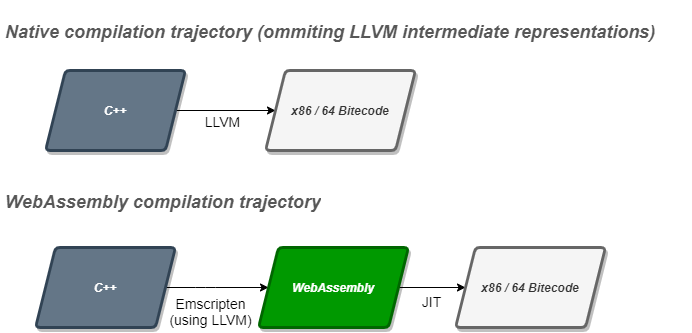
\includegraphics[width=\textwidth]{../schemas/wasm-performance/wasm-perf.png}
%     \caption{Comparison of compilation trajectories}
%     % based on the finding of \cite{jangda_not_2019}
%     \label{fig:wasm-trajectory}
%   \end{minipage}
% \end{figure}

% \subsubsection*{Adoption \& Implementation}

% not in a vaccuum

% On 5 December 2019, the \ac{w3c} officially pronounced WebAssembly as the fourth programming language of the web \cite{w3c_world_2019}. Philippe Le Hégaret, the \ac{w3c} Project Lead, writes “The arrival of WebAssembly expands the range of applications that can be achieved by simply using Open Web Platform technologies. In a world where machine learning and Artificial Intelligence become more and more common, it is important to enable high performance applications on the Web, without compromising the safety of the users,”. Since then, most major browsers have added official WebAssembly support.

% As of writing this proposal, WebAssembly has of yet not seen widespread adoption in web developer communities. Opinions deviate, but in general, WebAssembly is considered a niche technology, often being named as 'experimental' and 'bleeding edge'. 

% This would explain why, to the best of the author's knowledge, not many projects and papers explicitly link WebAssembly and GIS. Papers on \ac{wasm} do state \textit{"3d data transformations and visualization"} as some of the examples of a high performance web applications \cite{haas_bringing_2017, jangda_not_2019}. What's more, certain GIS applications, like Google Earth, have started to use WebAssembly, as seen in \reffig{fig:google-earth} \cite{google_google_2020}. How it is used is unknown due to the engine being closed-source, but it is speculated that \ac{wasm} is used to access code written for the original C++-based desktop application.

% \begin{figure}[!tbp]
%   \centering
%   \begin{minipage}[b]{0.80\textwidth}
%     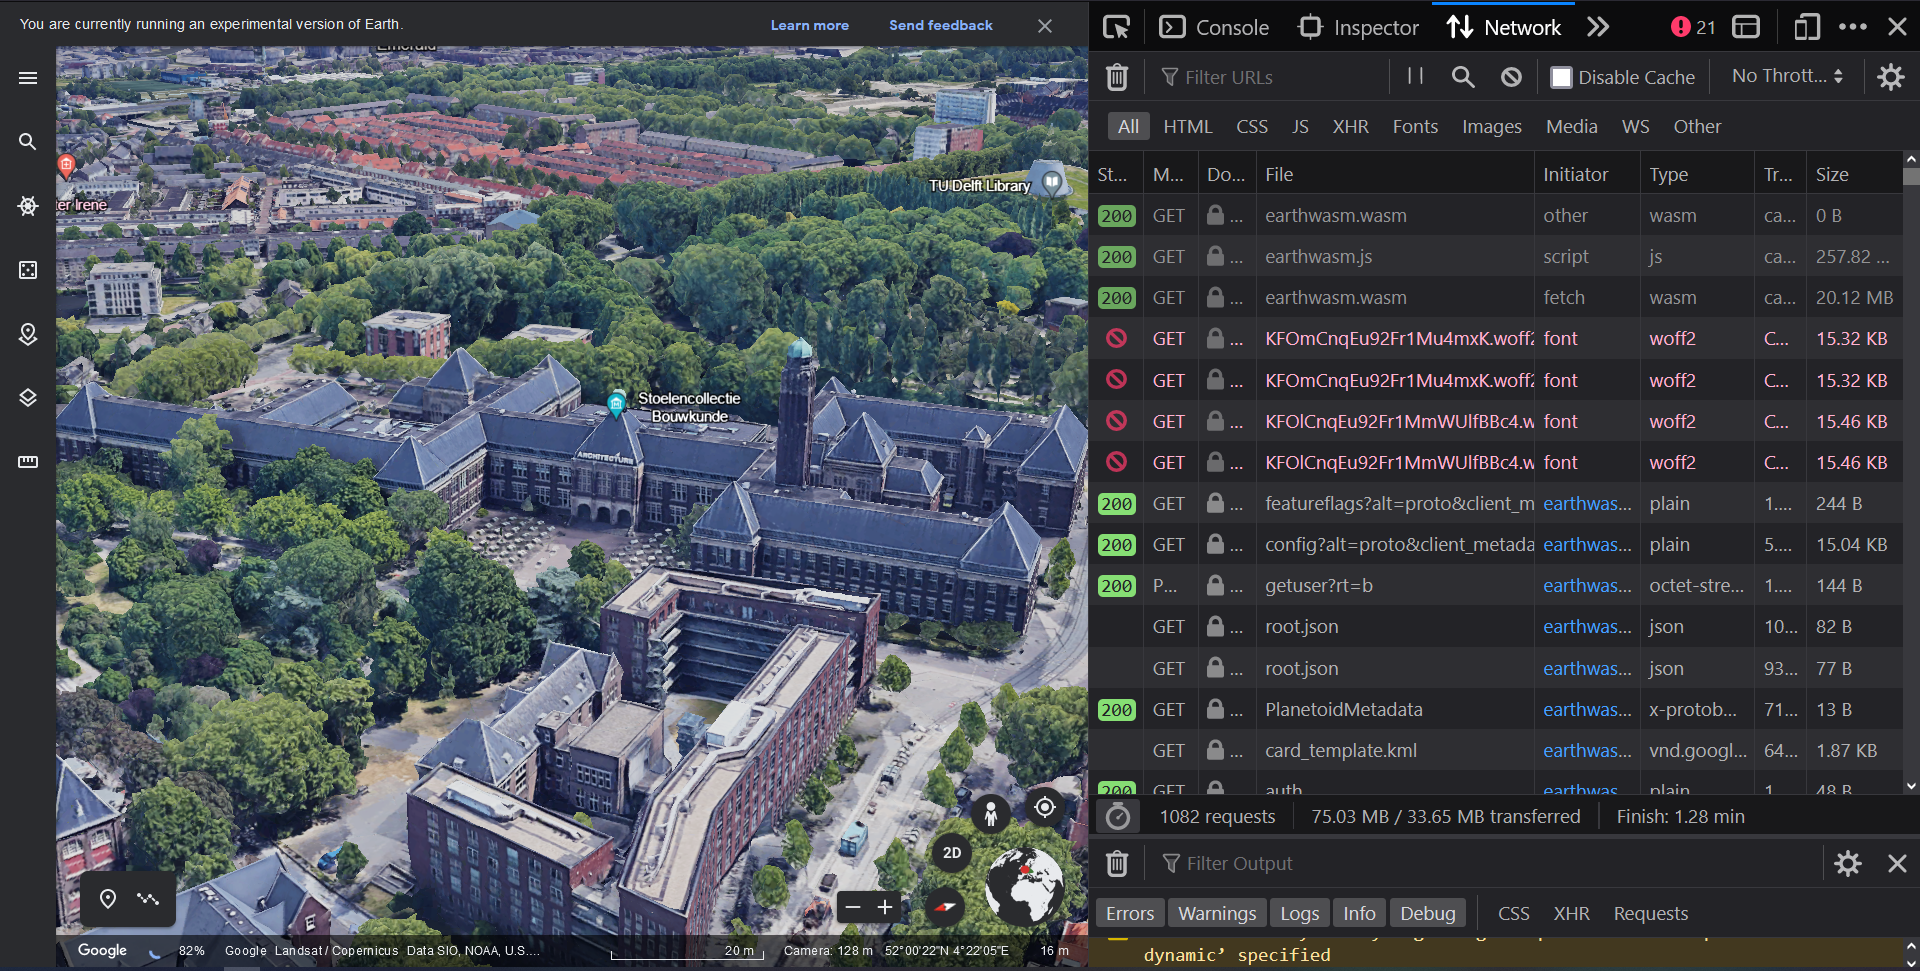
\includegraphics[width=\textwidth]{../images/google-earth-uses-webassembly.PNG}
%     \caption{Google Earth utilizing WebAssembly. Source: \cite{google_google_2020}}
%     \label{fig:google-earth}
%   \end{minipage}
% \end{figure}

% Some studies have taken place evaluating \ac{wasm}'s performance for geospatial operations specifically. Melch performed extensive benchmarks on polygon simplification algorithms written in both javascript and WebAssembly \cite{melch_performance_2019}. It concludes by showing WebAssembly was not always faster, but considerably more consistent. Melch had this to say: "To call the WebAssembly code the coordinates will first have to be stored in a linear memory object. With short run times this overhead can exceed the performance gain through WebAssembly. The pure algorithm run time was always shorter with WebAssembly.". These findings match \cite{jangda_not_2019}, showing that sometimes the javascript JIT compilers of especially the chromium implementation outperform WebAssembly, mainly because of these types of linear memory overhead.

% Lastly, the sparse matrix research of Sandhu et al. will be mentioned. \cite{sandhu_sparse_2018}. It shows again that WebAssembly's performance gain is most notable when performing scientific computations. it states: "For JavaScript, we observed that the best performing browser demonstrated a slowdown of only 2.2x to 5.8x versus C. Somewhat surprisingly, for WebAssembly, we observed similar or better performance as compared to C, for the best performing browser.". It also shows how certain preconceptions must be disregarded during research. For example, it turned out that for WebAssembly and JavaScript, double-precision arithmetic was more performant than single-precision.

% A recent study concerned with watershed delineation \cite{sit_optimized_2019} also concluded client-side WebAssembly to be more performant than server-side C, which, as a side effect, enabled their application to be published on the web. 

% On the topic of WebAssembly, the most important conclusion to to take away from prior research is \ac{wasm} must not be regarded as a 'drop-in replacement', as \cite{melch_performance_2019} puts it. Just like any language, WebAssembly has strengths and weaknesses. While \ac{wasm} is designed to be as unassumptious and unopinionated about its source language as possible, the implementations of host environments do favor certain programming patterns and data structures over others, and this will have to be taken into account during the proposed study.

%%%%%%%%%%%%%%%%%%%%%%%%%%%%%%%%%%%%%%%%%%%%%%%%%%%%%%%%%%%%%%%%%%%%%%%%%%%%%%%

% Based on the studies on WebAssembly, we can conclude that the compilation peculiarities of WebAssembly have to be taken into account, as it cannot be regarded as a 'drop in replacement'. There is also a significant difference between using WebAssembly theoretically, and using it realistically. The studies on Client-side geoprocessing tell us that these implementation details can have vast consequences on user experience, and studies on the Geoweb express that this user experience is vital to FAIR, cross-community geoprocessing.

% What this means for the methodology, is that a significant portion of this study's attention will have to go to experimenting with different ways of compiling to WebAssembly, while making sure it can still be used in a realistic scenario.
% If it turns out that the use-case app can only be used by experienced end-users who take special \ac{wasm} considerations in mind, a big reason of using the web, namely its accessibility, would be lost.  


%%%%%%%%%%%%%%%%%%%%%%%%%%%%%%%%%%%%%%%%%%%%%%%%%%%%%%%%%%%%%%%%%%%%%%%%%%%%%%%
\subsubsection{(More on webassembly)}

Not just open source: process sharing using fully containerized instances. Think .

current vision / direction: containerized, sharable processes, together with web-based, front end visual programming environments ( RasterFoundry). Docker is usually named as a vision for these sharable processes.

\m{->} We do have examples of cloud-native geodata formats, and some examples of cloud-based geo-computation (RasterFoundry , Google Earth Engine, more). However, these approaches have not yet tried to use truly sharable, containerized geoprocesses using Docker or WebAssembly. 

\m{->} WebAssembly as a whole is underresearched. WebAssembly is not a fully virtualized container image, but just a binary set of instructions, meant to be executed on a virtual machine. Think of safe, cross-platform dll's. 
WebAssembly is in this regard more simple than docker, but this gives it more opportunities. 
WebAssembly runs in the browser for instance. 

\m{->} This opportunity to run in the browser would enable these cloud-native frontend environments to "dry-run" these processes from within the browser, completely detached from the server, as a means to experiment with processes on a small scale before applying them to a cloud native environment. 

\m{->} However, no implementations exist yet which combines containerized processes with these frontend computation environments. 



% # 2. BACKGROUND

% ## 2.1 The Web Browser & JavaScript
% -  main players (chrome, safari, firefox, edge(==chrome))
% - The browser js speed armsrace
% - How that lead to WebAssembly

% ## 2.2 The Geospatial Web. 
% [Still relevant]

% ## 2.3 Related works on visual scripting
% - FME
% - GEOFLOW
% - OPENSCAD
% - Grasshopper

% ## 2.4 Related works on Demo Hosts


% ## 2.5 Client-side geoprocessing 
% [Still relevant]
% ...
% BUT: most of these studies were conducted before the increase in javascript performance described in 2.1. It is therefore a valid endeavor to retry the effort of client-side geoprocessing. 

% ## 2.6 Client-side Web Technologies 
% What do we mean with this term: 
% - HTML5 
% - WebGL
% - The Canvas API
% - WebWorkers 
% - WebAssembly 
% - WebComponents

% ### HTML5
% - leaflet

% ### WebGL
% - three.js
% - Celsium

% ### WebAssembly 
% [Might not be relevant]
% WebAssembly is since 2020 part of core web technologies

% ...

% 2 biggest reasons against client-side geoprocessing: 
% - not performant enough
% - no equivalent to industry-standard libraries (CGAL / GDAL). 

% WebAssembly COULD solve both, so this study includes WebAssembly as 


% <br><br>

% .....

%%%%%%%%%%%%%%%%%%%%%%%%%%%%%%%%%%%%%%%%%%%%%%%%%%%%%%%%%%%%%%%%%%%%%%%%%%%%%%%
\subsubsection*{Browser based geoprocessing software}

% https://www.azavea.com/blog/2016/09/26/raster-foundry-model-lab-phase-ii-sbir/
% https://geotiff.io/
- >
% https://www.eclipse.org/community/eclipse_newsletter/2018/december/geotrellis.php 
% -> ModelLab
% -> " Online tool to build, store, and execute complex geospatial models "
% - Mobius Modeller : https://mobius.design-automation.net/pages/mobius_modeller.html
% - GeoTIFF : https://app.geotiff.io/
These are all similar efforts, also hooked up to the OGC cloud native developments
Geofront will differ, for it focusses on 3D \& Point clouds instead of rasters \& map algebra, and focusses on client-side geodata consumption \& processing instead of being a server-side pipeline configurer.

ModelLab says this : "Widespread access to frequent, high-resolution Earth observation imagery has created the need for innovative tools like ModelLab that will help individuals and organizations to effectively access, analyze, edit, and visualize remotely sensed data in transformative new ways without years of specialized training or ongoing investments in proprietary software and technology infrastructure. "


%%%%%%%%%%%%%%%%%%%%%%%%%%%%%%%%%%%%%%%%%%%%%%%%%%%%%%%%%%%%%%%%%%%%%%%%%%%%%%%
\subsubsection*{Client-side geoprocessing}

% NEW PRACTICAL ATTEMPT. WHY? 
% - csg still has a lot of potential
% - previous studies:
%   - are dated
%   - prioritized theory over practicalities
%   - utilized the web's major feature of Accessibility and the clients feature of    
%     Interactivity inadequately 
%   - were not creative enough in terms of possible use-cases 

While these studies pose a strong theoretical case for client-side geoprocessing, their practical implementations were less convincing \todo{TODO: Figure out how to phrase this better}. 
The implementations of \cite{panidi_hybrid_2015, hamilton_client-side_2014} were written in a time before WebAssembly \& major javascript optimizations, and the study of \cite{kulawiak_analysis_2019} prioritized theory over practice. 


This study recognizes a need for a new, practical attempt at client-side geoprocessing. 
Client-side geoprocessing is a promising prospect with potentially many use cases.
Previous attempts are either dated due to the web's rapid advancements, or chose theory over practice.

In addition, the implementations lacked creativity \todo{This needs a better phrase, but it really is the most direct way of putting it}. 

The applications were either meant as small demo's, without a clear target audience or use-case in mind (just a way to demo performance), or as highly specified debugging tool for the authors.   
But, as mentioned before, a major advantage of Web applications over native applications is \emph{Accessibility}, and a major advantage of client-focussed web apps over server-focussed web apps is \emph{Interactivity}. 
By creating a client-side web application which is neither accessible nor interactive, the main incentive for creating a client-side web app is lost.
Additionally, by forgoing the question of accessibility, many auxiliary use-cases of client-side geoprocessing where overlooked.

%%%%%%%%%%%%%%%%%%%%%%%%%%%%%%%%%%%%%%%%%%%%%%%%%%%%%%%%%%%%%%%%%%%%%%%%%%%%%%%
\subsubsection*{The Cloud Native Geospatial movement}


% Establish OGC in two sentences, mentioning their name and Vision
The Open Geospatial Consortium (OGC)...
Mission: FAIR Geodata 

% Establish Cloud Native movement.
% GIS as one big LAN party
A prominent development within the OGC is the recent effort towards a \textbf{"Cloud Native Geospatial"} future. 
This initiative aims to radically simplify geodata storehouses to static servers serving large, singular binary geodata files. All processing and analysis of this geodata can then be performed by separate cloud-based web services. 
This architecture has many advantages over current geodata storage and analysis methods:
\begin{itemize}
  \item These new Cloud Native geodata formats are much cheaper to access by front-end and back-end services, compared to active services.
  \item Substituting active SQL or noSQL databases by static binary files is easier and cheaper for data providers, leading to more and more readily available geodata.
  \item By using supercomputers (Microsoft Planetary Computer) and cloud-storage (AWS), Geodata processes could make use of near-infinite computational and storage resources. 
  \item By having all data centralized in one location or type of location, new, large scale patterns within our geodata could be discovered.  
  \item For web GIS, this would offer direct data streaming options, similar to services like "Netflix" or "Spotify".  
\end{itemize}

These features may have a far reaching impact on society. Chris Holmes, forerunner of the cloud-native geospatial movement, envisions what the movement could mean for even non-GIS users: 
\emph{
  With the introduction of accessible, centralized data, and the dramatically different workflows that follow, Cloud Native Geospatial has the potential to introduce new, non-specialized users to the power of geospatial information that GIS practitioners have enjoyed for decades. [...]. The ecosystem of geospatial experts will collaborate to create analyses and insight, but any non-expert user will be able to select and apply those to the geographic area they care about. \~ Chris Holmes
}
% This is also reflected by cloud-native based tools like (Google Earth Engine or RasterFoundry) may achieve such a feed, by being web based and stuff...
All these reasons explain why the OGC and many other parties are now actively pursuing this vision.

But while this vision is in active development, many large-scale challenges are still in its way. 
One of the most important challenges is the required paradigm shift within geo-computation / geoprocessing workflows. 
The current, common geo-computation workflow of retrieving online data, only to run it through a local process and send the resulting data back into servers, will have to be reversed: In a cloud-native future, we will not retrieve data for our local process, but we will upload our process to the data.  
This introduces a sizable challenge: \textbf{Portable, Containerized Geo-computation}.

% \textbf{and the algorithms powering the processing can be shared online and customized collaboratively}. -> Chris again


% \begin{itemize}
%   \item Up to this point, the world of GIS has done a considerable effort to make geodata more Findable, Accessible, Interoperable, and Reusable. The challenge of Portable geo-computation now forces us to extend the effort of FAIR geodata to FAIR geodata computation as well.  
%   \item If we want our geodata processes to be just as portable as the geodata it takes as input, then perhaps the FAIR paradigm should extend from FAIR geodata to FAIR geodata processing . FAIR geo-computation.
%   \item Furthermore, it remains a mystery how these containerized containerized processes will be configured and accessed by frontend computation environments. 
%   \item Holmes: one of the vital ingredients: \emph{"and the algorithms powering the processing can be shared online and customized collaboratively"}.
% \end{itemize}

The challenge of sharing and chaining together containerized fragments of geoprocesses to a variety of environments will require more than just open source collaboration. 
This study interprets the challenge of portable geo-computation by means of the FAIR paradigm. 
If geodata processes need to be just as portable as the geodata forming the input and output, then perhaps the FAIR paradigm should extend from FAIR geodata to FAIR geodata \emph{processing} as well.
The challenge facing the cloud-native vision then becomes: \textbf{How to make geo-computation Findable, Accessible, Interoperable, and Reusable?} 
This links back to containerization, for containerization is a very powerful method of making geo-computation more Interoperable and Reusable.



% state of the art regarding this issue, make a path towards the particular thesis, and why it is an application
The current state of the art is far removed from either portable or FAIR geo-computation. 
\todo{Improve this intro}
\begin{itemize}
  \item current methods: Docker, and some geo-computation platforms.
  \item Not many implementations using WebAssembly, while this is a prime candidate: Even the guy who made Docker said so. 
  \item ignore the cloud: focus on the act of containerizing geoprocesses using webassembly an sich
\end{itemize}

FAIR geoprocessing may have many auxiliary advantages. 

% \begin{itemize}
%   \item Findable? -> web browser / Package Managers
%   \item Accessible? -> web tools
%   \item Interoperable -> WebAssembly / containerized runtimes and processes, using common types
%   \item Reusable -> compile to regular web service / function
% \end{itemize}

% X : wasm-based geo-computation applications

CITYJSON VALIDATOR ARGUMENT: THE WEB CAN BE USED TO IMMEDIATELY MAKE SOME TOOL / SOME RESEARCH PROJECT OPERATIONAL 'IN THE REAL WORLD'. THIS WAY, DATA CAN BE GATHERED, USER FEEDBACK CAN BE GATHERED, AND THE TOOL CAN BE EVALUATED IN TERMS OF REPRODUCABILITY. FINALLY, IT OFFERS THE POSSIBILITY OF THE TOOL BEING ACTUALLY USED, IN PRACTICE. 
z



\subsection*{REVIEW}

challenges
\begin{lstlisting}
Relevant Challenges & developments within web GIS:
- cloud-native movement
- 

\end{lstlisting}



acknoledgements
- Name similar studies or things 
  - Ravi Peter: awesome c++ based application 
    - not web
    - not formal reseach
  
%%%%%%%%%%%%%%%%%%%%%%%%%%%%%%%%%%%%%%%%%%%%%%%%%%%%%%%%%%%%%%%%%%%%%%%%%%%%%%%%


%%%%%%%%%%%%%%%%%%%%%%%%%%%%%%%%%%%%%%%%%%%%%%%%%%%%%%%%%%%%%%%%%%%%%%%%%%%%%%%
%%%%%%%%%%%%%%%%%%%%%%%%%%%%%%%%%%%%%%%%%%%%%%%%%%%%%%%%%%%%%%%%%%%%%%%%%%%%%%%
%%%%%%%%%%%%%%%%%%%%%%%%%%%%%%%%%%%%%%%%%%%%%%%%%%%%%%%%%%%%%%%%%%%%%%%%%%%%%%%
\section{The overlap of Visual Programming \& Web GIS}
\label{sec:both}

\subsection{Background}

\subsection{Review}